\chapter{Contexte du projet}
Cette partie présente le contexte du projet, le problème à traiter et les travaux existants au début de ce projet.


\section{Contexte du problème}
Depuis la démocratisation du concept de Cloud, plus en plus d'entreprises et organisations tendent à confier leurs applications aux fournisseurs de plateforme Cloud. En faisant ça, les entreprises n'ont pas besoin d'acheter et de maintenir leurs propres matériels, l'environnement fourni par les fournisseurs est prêt à l'emploi et largement personnalisable.


Sur le côté des fournisseurs (Amazon et Google par exemple), ils ont construit leurs super data centres pour avoir une puissance de calcul considérable et suffisante pour de nombreux clients. Par exemple pour Amazon Cloud Computing, selon une recherche effectuée en 2013 par l'entreprise NetCraft\footnote{\label{fn1}\url{http://news.netcraft.com/archives/2013/05/20/amazon-web-services-growth-unrelenting.html}}, le nombre des serveurs Amazon destiné aux applications web a atteint 158 mille.
\bigskip
\begin{figure}[!htbp]
	\centering
		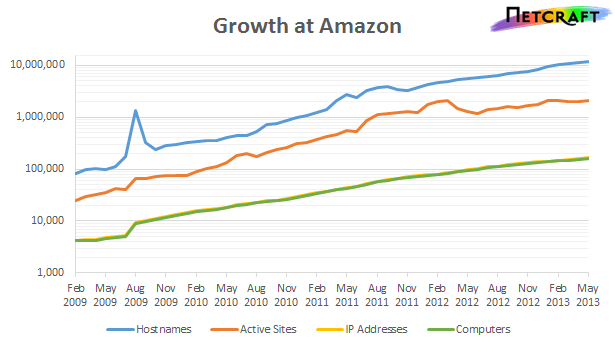
\includegraphics[scale=0.8]{pics/AMZN-growth.png}
	\caption{Croissance chez Amazon\ref{fn1}}
	\label{fig:amazon-growth}
\end{figure}
\bigskip


Ayant tellement nombreux de serveurs en utilisations, le coût généré devient énorme, seulement le coût de consommation d'électricité est déjà considérable. Les fournisseurs sont donc obligés d'optimiser chaque phase de production pour minimiser le coût. 

Avec la technologie de virtualisation, chaque tâche de client est considérée comme une machine virtuelle, plusieurs tâches peuvent s'exécutent en même temps sur une seule machine physique. Alors on a maintenant une question d'ordonnancement: à l'instant donné, quelle tâche doit être exécutée sur quelle machine? Cette question n'est pas facile à répondre à cause de nombreuses contraintes à respecter, qui seront expliquées dans la section suivante.


\section{Description du problème}
Ayant présenté le contexte du problème à traiter, dans cette partie, on va expliquer un peu en détail le problème en introduisant les contraintes à respecter et les objectifs à atteindre. Ils seront décrits d'une façon moins rigoureuse pour être plus compréhensible. La modélisation mathématique du problème peut être trouvée dans le chapitre suivant.


Les tâches seront placées sur des machines connectées en respectant les contraintes suivantes:


\subsection{Contraintes de préaffectation}
Il existe des contraintes qui influence directement sur le résultat de l'ordonnancement:
\bigskip
\begin{enumerate}
	\item Une tâche est planifiée d'être exécutée sur certains instants de temps.
	\item Une tâche ne peut être exécutée que sur certaines machines physiques.
\end{enumerate}
\bigskip

\subsection{Contraintes sur l'utilisation de machines}
Pour héberger une tâche, la machine doit avoir assez de ressources (CPU, GPU, RAM, HDD).


Une tâche peut être migrée d'une machine à l'autre, pendant la migration cette tâche utilise les ressources de toutes ces 2 machines. Puisque la migration est effectuée en parallèle de l'exécution de la tâche sur la machine de source, alors seulement les tâches qui ont été exécutée pendant assez de temps peuvent être migrées.


Une tâche qui est planifiée d'être exécutée peut éventuellement être suspendue si elle est du type préemptable. Pour réveiller cette tâche, il faut d'abord la recharger, ceci va prend du temps.

\subsection{Contraintes sur l'utilisation de réseaux}
Il peut y avoir des affinités entre les tâches. En ce cas, les tâches concernées ont besoin de communiquer entre elles pendant exécution, alors la bande passante du réseau doit être suffisante pour cette communication.



\subsection{Objectifs}
Il y a 2 objectifs à atteindre: minimisation du coût total et minimisation de la durée de reconfiguration.

Pour le premier, voici les coûts qu'on doit considérer:
\bigskip
\begin{itemize}
	\item Le coût d'utilisation des ressources (CPU, GPU, RAM, HDD) de machines.
	\item Le coût de suspension de tâches.
	\item Le coût de rester allumé pour les machines. On peut le considérer comme le coût de consommation. \end{itemize}
\bigskip




\section{Eléments existants}
Dans cette partie on va présenter le travail qui a déjà été réalisé avant ce projet.

\subsection{Modélisation mathématique}
Le modèle mathématique du problème a déjà été créé par Vincent T'Kindt et ses collègues. Toutes les contraintes ainsi que les fonctions objectifs sont déjà représentées sous forme de formulaire. Cette modélisation peut être transmise directement en programme CPLEX, qui peut ensuit trouver la solution optimale.


Le modèle complet peut être trouvé dans le chapitre suivant.

\subsection{Programme de la méthode exacte}
Le programme qui exprime le problème selon le modèle et qui utilise la librairie CPLEX pour trouver la solution optimale a déjà été réalisé par Vincent T'Kindt. Néanmoins, le problème étant prouvé NP-complet, quand on a une grande instance du problème, le programme CPLEX a besoin d'énormément de temps pour trouver une solution. Pour cette raison, on a besoin de chercher une approche heuristique, qui nous permet de trouver très vite une solution assez bonne mais pas forcément optimale.


Même si ce programme CPLEX qui est une approche exacte, n'est peut-être pas très adapté pour les gros instances du problème, il est indispensable dans le test, pour donner la solution optimale qui nous sert ensuite d'évaluer les appoaches heuristiques.


\subsection{Programme de la méthode heuristique}
Une première approche heuristique de liste a été aussi réalisée dans le cadre de PFE (2012 - 2013) de Cyrille PICARD. L'idée de l'approche et les algorithmes concernés ont été decrits dans son rapport de PFE. Par contre, à cause de la complexité du problème et la limite du temps, son implémentation contient des bugs qui rendent le programme incorrect. Alors sur la base de ce programme, j'ai essayé dans un premier temps de corriger les erreurs trouvées et d'améliorer cette implémentation.


\subsection{Programme testeur}
Un testeur a été aussi réalisé par Vincent T'Kindt. Ce testeur contient une partie de génération des instances de problème qui couvre 6 scénarios. Pour chaque instance de problème généré, le testeur appelle le programme de résolution pour trouver la solution et faire des statistiques sur les résultats obtenus.

